\documentclass[12pt,UTF8]{ctexbook}
\usepackage{ctex}
\usepackage{graphicx}
\usepackage{caption}
\usepackage{float}
\usepackage{wrapfig}
\usepackage{array}
\usepackage[table, dvipsnames, svgnames, x11names]{xcolor}
\usepackage{colortbl}% 
\usepackage{tabularx}
\usepackage{amsmath}
\usepackage{amssymb}
\usepackage{xfrac}
\usepackage{eucal}
\usepackage{titlesec}
\usepackage{amsthm}
\usepackage{tikz-cd}
\usepackage{enumitem}
\usepackage{verbatim}
\usepackage{fontspec,xunicode,xltxtra}
\usepackage{xeCJK} 

\definecolor{gl}{RGB}{246, 252, 240}
\definecolor{gd}{RGB}{236, 244, 230}
\definecolor{bg}{RGB}{242, 244, 228}


\setCJKmainfont[BoldFont=STZhongsong]{STSong}
\setCJKmonofont{simkai.ttf} % for \texttt
\setCJKsansfont{simfang.ttf} % for \textsf
\setlength\parskip{8pt}
\setlength{\fboxsep}{12pt}
\renewcommand\thesection{\arabic{chapter}.\arabic{section}}
\newtheorem{df}{定义}[section] 
\newtheorem{pp}{命题}[section]
\newtheorem{tm}{定理}[section]
\newtheorem{ex}{例子}[section]
\newtheorem{sk}{思考}[section]
\newtheorem{po}{公理}
\newtheorem*{so}{解答}
\newtheorem*{proof2}{证明}
\newtheorem{xt}{习题}[section]
\newtheorem{cor}{推论}[pp]
% 列举环境的行间距
\setenumerate[1]{itemsep=0pt,partopsep=0pt,parsep=0pt,topsep=0pt}
\setitemize[1]{itemsep=0pt,partopsep=0pt,parsep=0pt,topsep=0pt}
\setdescription{itemsep=0pt,partopsep=0pt,parsep=0pt,topsep=0pt}
\setlength{\intextsep}{2pt}%
\setlength{\columnsep}{2pt}%
% 新函数
\renewcommand\parallel{\mathrel{/\mskip-4mu/}}
\newcommand{\arcangle}{\mathord{\mathpalette\doarcangle\relax}}
\newcommand{\doarcangle}[2]{%
  \hbox{%
    \sbox0{$#1B$}%
    \sbox2{$#1<$}%
    \raisebox{\dimexpr\dp0+(\ht0-\ht2)/2}{%
      $#1<\mspace{-9mu}\mathrel{)}\mspace{2mu}$%
    }%
  }%
}
% 章节字体大小
\titleformat{\section}{\zihao{-2}\bfseries}{ \thesection }{16pt}{}
% 封面
\title{\zihao{0} \bfseries 极简数学·中学篇 \\ 第二册}
\author{\zihao{2} \texttt{大青花鱼}}
% \date{\bfseries\today}
\date{}
% 正文
\begin{document}
\maketitle
\tableofcontents
\newpage

\chapter{平面的形状}

生活中,很多东西形状有相似之处:
月亮和瓶盖、书本和书柜、电线杆和铅笔……
从“事物的多少”中,我们总结了数的概念;从“事物的形状”中,我们可以总结出形的概念。

我们生活的世界中有各种各样的事物,有遥远的星空,有脚下的大地,有宏伟的山川,有细小的花草。
四面八方,上下左右,各种事物之间位置不同。很长一段时期里,人们生活在地面上,认为大地是平的。
各种各样的事物都坐落在平坦的大地上。平面是人类最早总结出的概念之一。
古人很早就开始研究平面的形状,产生了最早的公理体系。

公理体系从几个最基本的假设和定义出发,认为这些假设和定义是不证自明的。依此推导对象的各种性质。
以下我们也试着用类似的方式,介绍平面上各种形状的性质。为了更好地理解以下的内容,我们建议你准备
一把刻度尺和足够的白纸。

\section{点、直线、线段、射线}
\textbf{点}是最基本的形,也是最特殊的形。点没有大小,没有形状,然而点是我们理解形状的基础。
我们一般用大写字母$A,B,C$等标记点。

点动起来就成了\textbf{线}。线没有宽度,只有长度。各种线中,\textbf{直线}是最基本的形。我们一般用小写字母$l,m,n$等标记直线。
\begin{po}{\textbf{直线公理}}\label{po:0}
    过不重合的两点有且仅有一条直线。
\end{po}
我们也说\textbf{两点确定一条直线}。两点$A,B$确定的直线称为直线$AB$。
$A,B$把直线分成三部分。$A,B$与它们之间的部分合起来,叫做\textbf{线段}$AB$或线段$BA$。$A$和$B$叫做线段的\textbf{端点}。
另外两部分分别叫做线段沿$A$和$B$的延长线。

直线$l$上一点$A$把直线分为两部分,称为点的两侧。点$A$与其中一侧合起来,叫做\textbf{射线}。
为了方便,我们也说$A$把$l$分成两条射线。$A$叫做射线的\textbf{端点}。
以$A$为端点,经过$l$上某点$B$的射线,可以叫做射线$AB$。

直线又把平面分为两部分,称为直线的两侧。给定一条直线,一点要么在直线上,要么在它两侧中的一侧。

两条直线要么\textbf{重合};要么恰好有一个公共点,称为\textbf{相交},这时公共点称为\textbf{交点};要么没有公共点,称为\textbf{平行}。
两条直线$l,m$平行,记为$l \parallel m$。
\begin{po}{\textbf{平行公理}}\label{po:1}
    过直线外一点,有且仅有一条与它平行的直线。
\end{po}
\begin{po}{\textbf{相交公理}}\label{po:2}
    两点分处某直线两侧,则它们确定的直线与其相交。
\end{po}
以上是一些基本概念和性质。公理体系中,它们分别叫做\textbf{公设}和\textbf{公理}。动手验证一下,这些概念和性质符合我们的直观感受吗?

\begin{sk}\label{sk:0-0-0}
    动手画一画,以下的说法对吗?\\
    1. 直线$AB$和直线$BA$是同一条直线。\\
    2. 射线$AB$和射线$BA$是同一条射线。\\
    3. 线段沿两端的延长线是射线。\\
    4. 线段$AB$是射线$AB$的一部分,线段$AB$和射线$AB$都是直线$AB$的一部分。\\
    数一数:\\
    1. 两点$A,B$把直线分成三部分,你能说出几条相关的射线?\\
    2. 平面上三点能确定几条直线?四点呢?\\
    3. 三条直线可以有几个交点?四条直线呢?
\end{sk}

\section{距离和长度}

生活中,我们经常接触到长度和距离的概念。比如,我们说“长江是中国最长的河流”,“上海和北京相距上千公里”等等。
什么是长度?什么是距离?

长度、位置和距离是密切联系的。我们用点表达位置,长度就是点运动产生的性质。
点的运动产生了长度,点的位置变化产生了距离。两点之间最短线的长度就是距离。对于直线和线段来说,长度和距离是相等的。
\begin{po}{\textbf{距离公理}}\label{po:3}
    两点之间线段最短。
\end{po}
两点确定的线段的长度就是两点的距离。我们用$ |\, \cdot\,|$符号表示长度,比如,线段$AB$的长度记作$|AB|$。
对线段来说,如果一条线段完全覆盖了另一条线段,
那么它不比另一条线段短。如果两条线段可以互相覆盖,就说它们等长。我们用“$=$”表示线段等长。

一般来说,位置不同的线段不一定互相覆盖。因此我们需要\textbf{等长公理}:
\begin{po}{\textbf{等长公理}}\label{po:4}
    \mbox{}\\
    \indent \textbf{5.1.} 给定两点$A,B$以及直线$l$,对$l$上任一点$C$,$C$两侧各有一点$D$,使得线段$|AB| = |CD|$。\\
    \indent \textbf{5.2.} 如果线段$|AB| = |CD|$,$|AB| = |EF|$,那么$|CD| = |EF|$。\\
    \indent \textbf{5.3.} 线段$AC$上有点$B$,线段$A'C'$上有点$B'$,且线段$|AB| = |A'B'|$,线段$|BC| = |B'C'|$,那么$|AC| = |A'C'|$。
\end{po}
第一条公理告诉我们,可以在任意直线的任意位置上复现一条等长的线段。第二条公理告诉我们长度和具体的线段无关,是普遍的性质。
第三条公理告诉我们长度可以相加。设线段$AC$上有一点$B$,我们说线段$AB$与线段$BC$(长度)之和线段$AC$(的长度)。
这样,给定了原点、单位长度和方向,我们就可以画出一条数轴了。

\section{角和角度}
点和线可以定义角的概念。角也是生活中常见的形状。钟面上的指针、桌椅的棱角、折扇的展开,都是角的形象。

一点发出的两条射线,就构成一个角。两条射线的公共端点叫做角的\textbf{顶点},其中一条射线叫做角的\textbf{始边},另一条叫做角的\textbf{终边}。

角有几种记法,取决于我们已知的信息。比如,如果我们知道角的顶点$O$和始边和终边上各一点$A,B$,可以把角记作$\angle AOB$。
其中$\angle$表示角的意思。如果已知角的顶点$O$,而且相关图形上显然只有一个以$O$为顶点的角,那么可以把角简记作$\angle O$。
如果不知道角的顶点,但相关图形上为角标示了记号,也可以直接使用这个记号。一般用小写希腊字母$\alpha, \beta, \gamma$或$1,2,3$等数字
标示角。

角与角之间可以比较大小吗?两个角的顶点、始边和终边都重合,就说两者相等。我们用“$=$”表示角相等。
对顶点和始边不重合的角,我们需要\textbf{等角公理}:
\begin{po}{\textbf{等角公理}}\label{po:5}
    \mbox{}\\
    \indent \textbf{6.1.} 给定$\angle AOB$和射线$O'A'$,总有唯一的射线$O'B'$使得$\angle A'O'B' = \angle AOB$。\\
    \indent \textbf{6.2.} 如果$\angle A = \angle B$,$\angle A = \angle C$,那么$\angle B = \angle C$。\\
    \indent \textbf{6.3.} 给定$\angle AOB$和$\angle BOC$。如果$\angle A'O'B' = \angle AOB$,$\angle B'O'C' = \angle BOC$,
    那么$\angle A'O'C' = \angle AOC$。
\end{po}
第一条公理告诉我们,可以从任何射线出发,复现一个角。第二条公理告诉我们,角的大小和顶点、射线的位置无关,是普遍的性质。
第三条公理告诉我们,角度可以相加。我们说$\angle AOB$与$\angle BOC$的和是$\angle AOC$,记作$\angle AOB + \angle BOC = \angle AOC$。

直线上一点把直线分为两条射线,于是形成一个角。这样的角叫做\textbf{平角}。
所有的直线都是一样的,于是所有的平角都一样大。始边和终边重合的角叫做\textbf{零角}。直观上看,零角就是一条射线。
所有的射线都是一样的,于是所有的零角都一样大。

如果$\angle AOB$不是平角,记直线$OA$被$O$分成射线$OA$和$OA'$,则$\angle BOA'$叫做$\angle AOB$的\textbf{补角}。

补角和自己一样大的角叫做\textbf{直角}。按照定义,一个平角等于两个直角。
如果$\angle AOB$是直角,那么$\angle AOC$和$\angle COB$互为\textbf{补角}。

\begin{wrapfigure}{r}{0.22\textwidth} %this figure will be at the right
    \vspace{-10pt}
    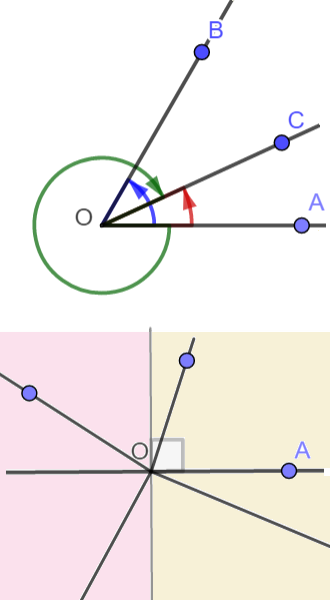
\includegraphics[width=0.22\textwidth]{角度1.png}
    % \captionsetup{labelformat=empty}
    % \caption{角的大小}
\end{wrapfigure}

如右图,$\angle AOB$和$\angle AOC$谁更大?$\angle AOC$到底指哪个角?

我们约定:\textbf{逆时针方向是正向}。始边逆时针方向旋转到终边形成的角是正的,否则是负的。
始边逆时针旋转到所在直线另一侧,形成平角;继续逆时针旋转到与自身重合,形成的角叫\textbf{周角}。
一个周角就是射线旋转一周,等于两个平角。相差一个或几个周角的角,形状是一样的。
我们可以约定只讨论负平角到正平角之内的角。如果某个角超过了这个范围,就相应加上或减去一个周角,
直到从始边到终边旋转不超过一个平角。

习惯上,我们把平角内部均匀分为$180$份,每份称为$1$度,也记作$1^\circ$。
周角是$360$度的角,平角是$180$度的角,直角是$90$度的角。
于是,每个角对应一个数,称为它的角度。角的大小,可以用角度来衡量。

给定直线$l$上点$O$为顶点的平角和对应的直角。直角所在的把平面分为两侧。
从平角的始边出发,终边和始边属于同侧的角,叫做\textbf{锐角};终边和始边分属两侧的角,叫做\textbf{钝角}。

量角器是日常用来衡量角度的工具。使用量角器,我们可以测量角的大小,也可以画出指定角度的角。

把平角$180$等分来表示角的大小,这种方法叫做\textbf{角度制}。除此以外,还有\textbf{弧度制}等其他方法表示角的大小。
\begin{sk}\label{sk:0-2-0}
    \mbox{}\\
    1. $470^\circ$的角是什么角?$4700^\circ$的角是什么角?画出两个角。谁比较大?\\
    2. 锐角和钝角的角度可以是多少?它们和直角的大小关系如何?\\
    3. 角度和长度有什么不同?为什么有这种不同?\\
    4. 如何把一个角分为两半?
\end{sk}

\chapter{直线与角的关系}
上一章我们学习了直线和角的概念。现在我们来看直线和角的关系。

\section{直线交角}
\begin{wrapfigure}[4]{r}{0.21\textwidth} %this figure will be at the right
    \vspace{-15pt}
    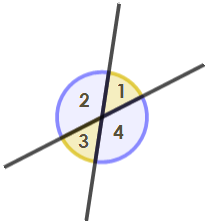
\includegraphics[width=0.21\textwidth]{角度0.png}
    % \captionsetup{labelformat=empty}
    % \caption{对顶角}
\end{wrapfigure}

如右图,两条直线相交于一点,分成四条射线。图中四个角有什么关系?

我们把处在$\angle 1$和$\angle 3$位置关系的一对角称为对顶角,$\angle 2$和$\angle 4$也是对顶角。
$\angle 2$既是$\angle 1$的补角,也是$\angle 3$的补角,所以$\angle 1 = \angle 3$。
同理,$\angle 2 = \angle 4$。也就是说:\textbf{对顶角相等}。

由于对顶角相等,我们可以定义直线的\textbf{交角}。$\angle AOB$始边所在直线$OA$逆时针旋转到与终边所在直线$OB$首次重合,形成的角称为
$OA$到$OB$的交角,记为$\arcangle AOB$。每个交角对应一对顶角。线段、射线与直线之间的交角,都定义为它们所在直线的交角。比如,线段与直线的交角,就是线段所在的直线与它的交角。

直线的交角总是正的,而且不超过平角。约定平行、重合的直线交角为平角。$\arcangle BOA$与$\arcangle AOB$互为补角。

一条直线到另一条直线的交角为直角,就说它\textbf{垂直}于另一条直线。这时,另一条直线到它的交角是直角的补角,因此也是直角。
于是我们说两者互相\textbf{垂直}。相互垂直的两条直线$l,m$记为$l\perp m$。


\section{同位角、内错角、同旁内角}
如右图,两条平行的直线和同一条直线相交,形成了八个角。这八个角之间有什么关系呢?

\begin{wrapfigure}{r}{0.4\textwidth} %this figure will be at the right
    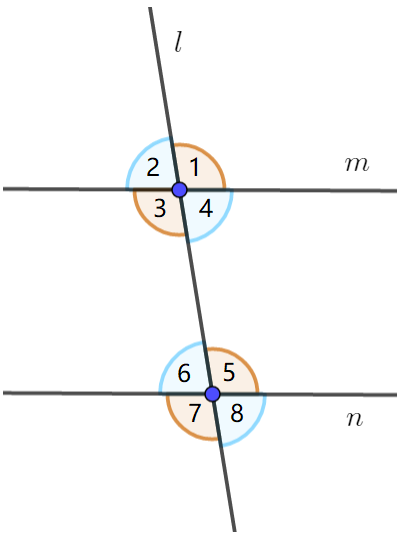
\includegraphics[width=0.4\textwidth]{三线八角.png}
\end{wrapfigure}

观察$\angle 1$和$\angle 5$,我们说这种位置关系的一对角是\textbf{同位角}。它们的终边属于同一条直线,始边属于两条直线交这条直线的同侧。
我们可以发现:\textbf{两条线平行时,同位角相等}。除了$\angle 1 = \angle 5$,还有:$\angle 2 = \angle 6$,$\angle 3 = \angle 7$,$\angle 4 = \angle 8$。

再看$\angle 3$和$\angle 5$,我们说这种位置关系的一对角是\textbf{内错角}。它们的始边属于同一条直线,终边属于两条直线交这条直线的异侧。$\angle 1 = \angle 3$,而$\angle 1 = \angle 5$,所以根据等角公理,$\angle 3 = \angle 5$。
所以,\textbf{直线截两条平行线,得到的内错角相等}。同理,$\angle 4 = \angle 6$。

最后来看$\angle 4$和$\angle 5$,我们说这种位置关系的一对角是\textbf{同侧内角}或\textbf{同旁内角}。一角的始边和另一角的终边属于同一条直线,该角的终边和另一角的始边属于两条直线交这条直线的同侧。
$\angle 4$是$\angle 1$的补角,
而$\angle 1 = \angle 5$,所以$\angle 4$与$\angle 5$加起来是平角。所以,\textbf{直线截两条平行线,得到的同旁内角和为平角}。

\begin{sk}\label{sk:1-1-0}
    \mbox{}\\
    1. $\angle 2$和$\angle 5$的大小有什么关系?$\angle 1$和$\angle 6$呢?\\
    2. $\angle 2$和$\angle 8$的大小有什么关系?$\angle 1$和$\angle 8$呢?\\
    3. 如果两条线不再平行,同位角、内错角和同旁内角还相等吗?
    4. 能不能用直线交角,解释同位角、内错角和同旁内角?
\end{sk}

同位角、内错角和同旁内角可以用来判断两条直线是否平行。如果两条直线平行,
那么同位角相等、内错角相等,同旁内角相加是平角。反过来,如果同位角相等、内错角相等,或者同旁内角相加是平角,
那么对应的两条直线平行。
% https://commons.wikimedia.org/wiki/File:Diyarbakir_1050645_Droste_Effect.jpg
\begin{wrapfigure}[6]{r}{0.225\textwidth} %this figure will be at the right
    \vspace{50pt}
    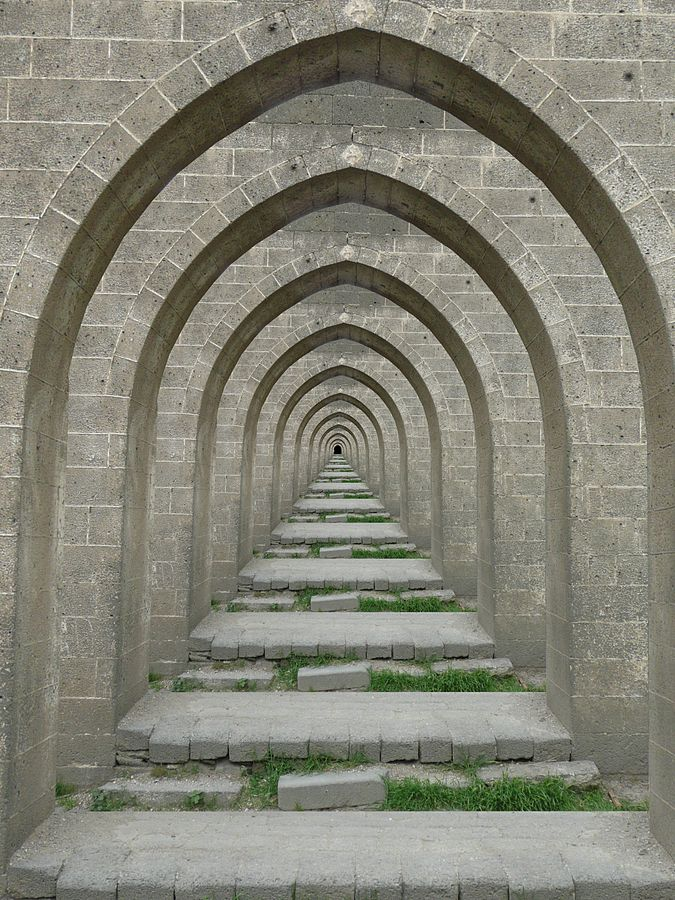
\includegraphics[width=0.225\textwidth]{675px-Diyarbakir_1050645_Droste_Effect.jpg}
\end{wrapfigure}

\section{相似和比例}
观察右图,各个拱门之间有什么关系?
两个图形可以形状一样,只有大小不同。
这样的关系,称为相似关系。

\begin{wrapfigure}{r}{0.24\textwidth} %this figure will be at the right
    \vspace{-15pt}
    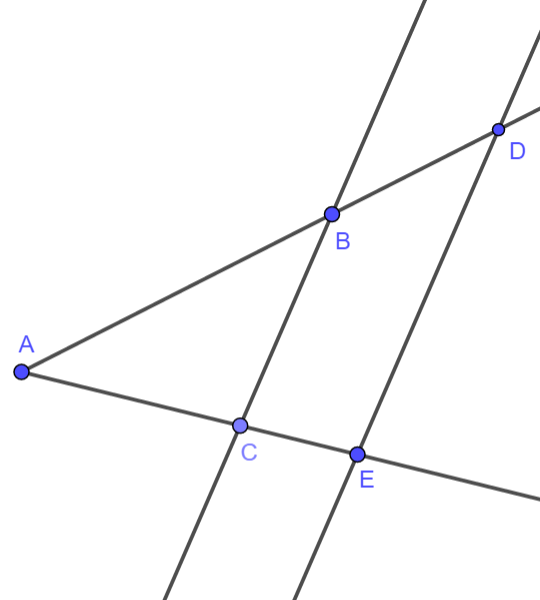
\includegraphics[width=0.24\textwidth]{比例1.png}
\end{wrapfigure}

用量角器测量相似图形相应位置的角度,以及相似部分的长度,你有什么发现?

相似的图形,对应部位的角度相等,长度成比例。

观察右图,从一点出发的两条射线和两条平行线相交。用刻度尺测量线段$AB$、$AD$、$AC$、$AE$、$BC$和$DE$的长度。你有什么发现?
\begin{po}{\textbf{放缩公理}}\label{po:6}
    从一点$A$出发的两条射线,每条线上取两点:$B,D$和$C,E$。如果
    $$ \frac{|AB|}{|AD|} = \frac{|AC|}{|AE|},$$
    那么,
    $$ \frac{|AB|}{|AD|} = \frac{|AC|}{|AE|} = \frac{|BC|}{|DE|},$$
    而且$\angle ABC = \angle ADE$,$\angle ACB = \angle AED$。
\end{po}
\begin{wrapfigure}{l}{0.24\textwidth} %this figure will be at the left
    \vspace{-10pt}
    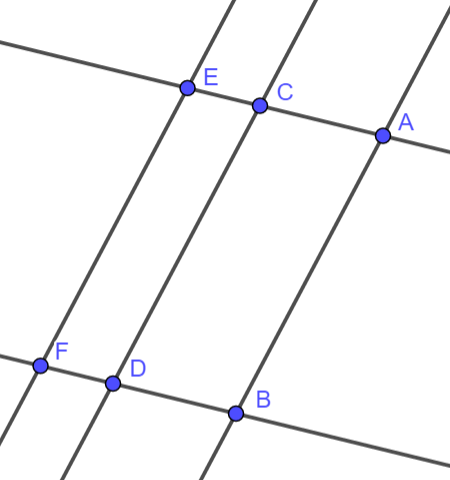
\includegraphics[width=0.24\textwidth]{比例2.png}
\end{wrapfigure}

注意到$\angle ABC$和$\angle ADE$是同位角,所以两者相等,就说明直线$BC$和直线$DE$平行。

\begin{sk}\label{sk:1-2-0}
    \mbox{}\\
    1. 如果一点$A$出发的两条射线$AB$、$AC$和两条平行线分别相交于$B,D$和$C,E$,那么线段$AB$、$AD$、$AC$、$AE$、$BC$和$DE$的长度有什么关系,如何证明?\\
    2. 如左图,直线$AB$、$CD$和$EF$平行,直线$AC$和$BD$平行。证明$|EC|$和$|CA|$之比等于$|FD|$和$|DB|$之比。\\
    3. 给定线段$AB$,如何找出它的中点?\\
    4. 给定直线$OA$,以线段$OA$长度为单位,$O$到$A$的方向为正方向,构建数轴。能否在数轴上找出长度为有理数$\frac{p}{q}$的线段$OB$?
\end{sk}

\chapter{判断和推理}
\section{充分条件和必要条件}
我们已经学过判断:\textbf{判断},是对事物情况表达肯定或否定的态度。判断包括简单判断和复合判断。
简单判断包括全判断、有判断和单判断,复合判断包括联言判断、或言判断、选言判断和假言判断。

假言判断是关于条件的判断,它涉及两个称为\textbf{前件}和\textbf{后件}的判断,并判断前件是后件成立的条件。
假言判断并不对前件或后件做判断,只对两者的条件关系做判断,而条件关系又分为两种:\textbf{充分条件}和\textbf{必要条件}。

充分条件假言判断想说的是:前件为真的时候,后件也为真。比如:人如果不吃东西,就会饿。
这个例子里,前件是“人不吃东西”,后件是“人会饿”。前件真的时候,后件也是真的,这说明充分条件关系是真的。
我们说,前件是后件的充分条件。这个例子里,“人不吃东西”是“人会饿”的充分条件。

\begin{sk}\label{sk:2-0-0}
    \mbox{}\\
    \indent “你要是考了满分,母猪都会上树了!”\\
    \indent 1. 这句话里,“你考了满分”和“母猪会上树”是什么关系?\\
    \indent 2. “你”如果没考满分,这个关系还成立吗?这时“母猪会上树”和“母猪不会上树”对这个判断有什么影响?
\end{sk}

充分条件判断的真值表为:
\begin{center}
    \begin{tabular}{ p{3em}<{\centering} p{3em}<{\centering} p{8em}<{\centering} }
        \rowcolor{gd} $p$ & $q$ & 如果$p$,那么$q$ \\ [0.5ex] 
        \noalign{{\color{white}\hrule height 2pt}} % \hline\hline
        \rowcolor{gl} 真 & 真 & 真  \\  
        \noalign{{\color{white}\hrule height 2pt}}% \hline
        \rowcolor{gd} 真 & 假 & 假  \\
        \noalign{{\color{white}\hrule height 2pt}}% \hline
        \rowcolor{gl} 假 & 真 & 真 \\  
        \noalign{{\color{white}\hrule height 2pt}}% \hline
        \rowcolor{gd} 假 & 假 & 真 \\
    \end{tabular}
\end{center}

必要条件假言判断想说的是:前件为假的时候,后件也为假。比如:人只有识字了,才能读书。
这个例子里,前件是“识字”,后件是“能读书”。不识字的人,不能读书。前件假的时候,后件也是假的,这说明必要条件关系是真的。
我们说,前件是后件的必要条件。这个例子里,“识字”是“能读书”的必要条件。

\begin{sk}\label{sk:2-0-1}
    \mbox{}\\
    \indent “只有到了晚上,才能看见满天的星星。”\\
    \indent 1. 这句话里,“到了晚上”和“看见星星”是什么关系?\\
    \indent 2. 有时,到了晚上也看不见星星。是否说明这个判断不成立呢?
\end{sk}

必要条件判断的真值表为:
\begin{center}
    \begin{tabular}{ p{3em}<{\centering} p{3em}<{\centering} p{8em}<{\centering} }
        \rowcolor{gd} $p$ & $q$ & 只有$p$,才有$q$ \\ [0.5ex] 
        \noalign{{\color{white}\hrule height 2pt}} % \hline\hline
        \rowcolor{gl} 真 & 真 & 真  \\  
        \noalign{{\color{white}\hrule height 2pt}}% \hline
        \rowcolor{gd} 真 & 假 & 真  \\
        \noalign{{\color{white}\hrule height 2pt}}% \hline
        \rowcolor{gl} 假 & 真 & 假 \\  
        \noalign{{\color{white}\hrule height 2pt}}% \hline
        \rowcolor{gd} 假 & 假 & 真 \\
    \end{tabular}
\end{center}

如果前件既是后件的充分条件,也是后件的必要条件,就说前件是后件的\textbf{充要条件}。
充要条件一般用“当且仅当”句式来表达。比如:“李四年纪比张三大,当且仅当张三年纪比李四小。”

充要条件假言判断可以看成充分条件假言判断和必要条件假言判断的联言判断。因此,充要条件判断的真值,
可以通过充分条件判断的真值和必要条件判断的真值得到:
\begin{center}
    \begin{tabular}{ p{3em}<{\centering} p{3em}<{\centering} p{7em}<{\centering} p{7em}<{\centering} p{7em}<{\centering} }
        \rowcolor{gd} $p$ & $q$ & 如果$p$,那么$q$ & 只有$p$,才有$q$ & $p$,当且仅当$q$ \\ [0.5ex] 
        \noalign{{\color{white}\hrule height 2pt}} % \hline\hline
        \rowcolor{gl} 真 & 真 & 真 & 真 & 真 \\  
        \noalign{{\color{white}\hrule height 2pt}}% \hline
        \rowcolor{gd} 真 & 假 & 假 & 真 & 假 \\
        \noalign{{\color{white}\hrule height 2pt}}% \hline
        \rowcolor{gl} 假 & 真 & 真 & 假 & 假 \\  
        \noalign{{\color{white}\hrule height 2pt}}% \hline
        \rowcolor{gd} 假 & 假 & 真 & 真 & 真\\
    \end{tabular}
\end{center}
可以看到,前件和后件都为真、都为假的时候,充要条件判断为真。前件和后件一真一假的时候,充要条件判断为假。

\begin{sk}\label{sk:2-0-2} 前件和后件互换位置,充要条件判断是否会变化?这说明了什么?
\end{sk}

\section{换质和换位}
上一节中,我们可以见到,判断之间在真假方面是有联系的。利用其中的规律,
我们可以通过已经知道真假的判断,得知另一些判断的真假。这种思考称为\textbf{推理}。
推理过程中,已经知道真假的判断,叫做\textbf{前提};通过思考得知真假的判断,称为\textbf{结论}。

有些推理是符合客观现实的,我们通过总结客观事物的性质,可以验证它们是有效的推理。另外一些推理不符合
客观事实,我们可以验证它们是无效的推理。

最简单的推理,是从一个简单判断到另一个简单判断的推理。我们称这种推理为\textbf{直接推理}。
\begin{sk}\label{sk:2-1-0} 
    以下的例子中,前后两句话有什么关联?\\
    \indent 1. 有的哺乳动物是非素食动物。有的哺乳动物不是素食动物。\\
    \indent 2. 所有个位是$3$的数都不是偶数。所有个位是$3$的数都是奇数。\\
    \indent 3. 这盒牛奶不是变质的。这盒牛奶是没变质的。
\end{sk}
以上每个例子中,前一句话和后一句话的区别在于:后一句话把前一句话的断语变成了与它矛盾的概念,然后把判断变成了对应的非判断。
比如,第三个例子中,后一句把“变质的”改成了矛盾的概念:“没变质的”,然后把否定句改成了肯定句。

我们发现,这种方法不会改变判断的真假。把判断改成非判断,同时把事物的性质改成矛盾的概念,判断的真假不变。
因此,把一个判断作为前提,把如上改变后的判断作为结论,就得到一个有效的推理。我们一般用“因为……所以……”、“……,因此……”等句式
描述推理。比如,对第三个例子,我们可以这么描述:

因为这盒牛奶不是变质的,所以这盒牛奶是没变质的。

我们把这种推理方法称为\textbf{换质法}。“质”指“肯定句”和“否定句”这两种形式,“换质”指从肯定换为否定或者从否定换为肯定。
\begin{xt}\label{xt:2-0-0}
    以下推理是不是有效的推理?为什么?\\
    \indent 1. 因为蚂蚁不是植物,所以蚂蚁是动物。 \\
    \indent 2. 因为这盒牛奶不是脱脂的,所以这盒牛奶是全脂的。 \\
    \indent 3. 因为有的条款不是不可逆的,所以有的条款是可逆的。 \\
    \indent 4. 因为有的董事会成员不反对转型方案,所以有的董事会成员反对不转型方案。
\end{xt}

\begin{sk}\label{sk:2-1-1} 
    以下的例子中,前后两句话有什么关联?\\
    \indent 1. 有的物理学家是共产主义者。有的共产主义者是物理学家。\\
    \indent 2. 所有的西瓜都是水果。所有的水果都是西瓜。\\
    \indent 3. 陈家洛是红花会的总舵主。红花会的总舵主是陈家洛。
\end{sk}
以上每个例子中,前一句话和后一句话的区别在于:后一句话把前一句话的断语变成了主语,然后把主语变成了对应的断语。
比如,第二个例子中,后一句把“水果”改成了主语,把“西瓜”改成了宾语。我们把这种操作称为\textbf{换位法},
即交换了判断的主语和断语的位置。

换位法是否改变了判断的真假?

第一个例子中,我们可以确信,只要第一句是真的,那么第二句就是真的。
如果有的物理学家是共产主义者,比如物理学家奥本海默是共产主义者,那么奥本海默这个共产主义者也的确是物理学家,
于是,有的共产主义者是物理学家。

第二个例子中,“所有的西瓜是水果”是真的,但“所有的水果是西瓜”是假的。比如苹果就不是西瓜。

第三个例子中,如果陈家洛是红花会的总舵主,那么红花会的总舵主是不是陈家洛呢?如果红花会的总舵主只有一个,
那么他就是陈家洛。如果红花会的总舵主不止一个,那么就不能说“红花会的总舵主是陈家洛”。

我们发现,换位法不总是有效的推理。什么时候,换位法有效呢?从前面的例子看出,换位法无效,总是因为前提里我们并没有在讨论某个概念的全体,
在结论里我们却在讨论它的全体。

比如,第二个例子里,前提“所有的西瓜是水果”中讨论了所有的西瓜,但并没有涉及水果这个概念的全体。
我们讨论这个判断的真假时,不需要检查每个水果。可到了结论里,我们却要讨论所有的水果。同样的,第三个例子里,
我们讨论“陈家洛是红花会的总舵主”时,并没有涉及所有的红花会总舵主,只讨论陈家洛是不是总舵主。其他总舵主,如果有的话,
并不在讨论范围内。而到了结论里,我们却要讨论“红花会的总舵主”全体了。

所以,换位法需要再加一条规则才是有效的推理:\textbf{前提中讨论的概念如果不涉及它的全体,结论中也不能涉及它的全体。}

我们把“概念涉及它的全体”称为概念\textbf{周延},把“概念不涉及它的全体”称为概念\textbf{不周延}。那么,
换位法缺的规则可以复述为:\textbf{前提中讨论的概念如果不周延,它在结论中也不周延。}

举例来说,前提“有的水果不是西瓜”换位到结论“有的西瓜不是水果”是无效的推理,因为前提中
“水果”不周延,而结论中,为了判断“不是水果”,我们需要检查所有的水果,结论中的“水果”周延。

对于主语来说,周延和全判断是一致的,不周延和有判断是一致的。全判断的主语是周延的,有判断的主语是不周延的。

对于断语来说,否定后接的断语总是周延的:为了否定一个性质,我们需要检查这个性质所有的个体。肯定后接的断语总是不周延的:
我们只需要对主语涉及的概念进行检查就可以了。比如,要判断“有的水果是西瓜”,我们只需要找一个是西瓜的水果就可以了;
而要判断“有的水果不是西瓜”,我们要确认给出的水果不是西瓜,就必须检查每个西瓜。

于是,换位法的规则又可以这么描述:
\begin{center}
    \fbox{
        \shortstack[l]{
            1. 全否定判断换位可以推出全否定判断。\\
            2. 单否定判断换位可以推出单否定判断。\\
            3. 有肯定判断换位可以推出有肯定判断。\\
            4. 单肯定判断换位可以推出单肯定判断。
        }
    }
\end{center}

\begin{xt}\label{xt:2-0-1}
    以下推理是不是有效的推理?为什么?\\
    \indent 1. 因为军国主义者是支持东南亚民族自决的,所以支持东南亚民族自决的是军国主义者。 \\
    \indent 2. 因为有的可解群是非交换群,所以有的非交换群是可解群。 \\
    \indent 3. 因为所有等温过程都不是等熵过程,所以所有等熵过程都不是等温过程。 \\
    \indent 4. 因为有的展品是非卖品,所以有的卖品不是展品。 \\
    \indent 5. 因为有的可解群是非交换群,所以有的交换群不是可解群。
\end{xt}

% \section{归谬法和反证法}
% 简单判断
% \begin{sk}\label{sk:2-1-1} 
%     以下的例子中,前后两句话有什么关联?\\
%     \indent 1. 有的物理学家是共产主义者。有的共产主义者是物理学家。\\
%     \indent 2. 所有的西瓜都是水果。所有的水果都是西瓜。\\
%     \indent 3. 陈家洛是红花会的总舵主。红花会的总舵主是陈家洛。
% \end{sk}


\chapter{全等三角形}
\section{认识三角形}
\begin{wrapfigure}[4]{r}{0.32\textwidth} %this figure will be at the right
    \vspace{-35pt}
    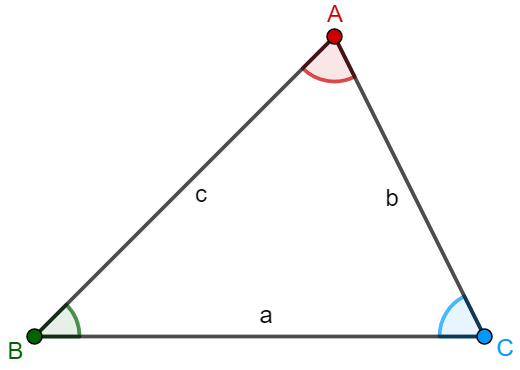
\includegraphics[width=0.32\textwidth]{三角形0.png}
\end{wrapfigure}
两点可以确定一条直线,三点可以确定什么呢?把三个点两两相连,得到三条线段。
我们把这样的形状称为\textbf{三角形}。点$A,B,C$确定的三角形称为“三角形$ABC$”,记为$\triangle ABC$。



点$A,B,C$称为三角形的\textbf{顶点},线段$AB$,$BC$和$AC$称为三角形的\textbf{边}。
射线$AB$和$AC$确定的角记为$\angle A$,类似有$\angle B$和$\angle C$,它们叫做$\triangle ABC$的\textbf{内角},
简称$\triangle ABC$的角。内角的补角称为\textbf{外角}。边$BC$称为$\angle A$的对边,$AB$和$AC$称为$\angle A$的邻边,$\angle A$称为$BC$的对角;
$\angle B$和$\angle C$也如是。

\begin{wrapfigure}[5]{l}{0.15\textwidth} %this figure will be at the right
    \vspace{-20pt}
    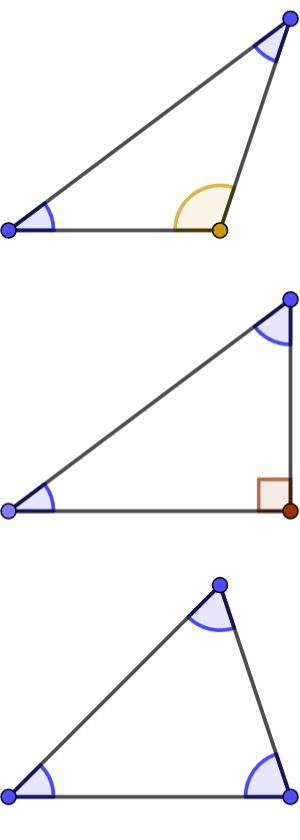
\includegraphics[width=0.144\textwidth]{三角形1.png}
\end{wrapfigure}

我们知道,三角形内角之和是$180^\circ$,也就是平角。因此:
\begin{itemize}
    \item 如果三角形有一个内角是钝角,那么另外两个角的和小于直角,这种三角形称为\textbf{钝角三角形}。
    \item 如果三角形有一个内角是直角,那么另外两个角的和等于直角,这种三角形称为\textbf{直角三角形}。
    \item 如果三角形内角中没有钝角也没有直角,这种三角形称为\textbf{锐角三角形}。
\end{itemize}

两点之间线段最短。所以,\textbf{三角形任何两边长度之和大于第三边。}

\section{判定全等关系}
线段之间有等长关系,角之间有相等关系,三角形之间也有全等的关系。如果两个三角形对应的边长度都一样,
对应的角形状也一样,就说这两个三角形\textbf{全等}。

判断三角形全等,我们有三角形的\textbf{全等公理}:
\begin{po}{\textbf{三角形全等公理}}\label{po:7}
    考虑$\triangle ABC$和$\triangle A'B'C'$。如果$|AB| = |A'B'|$、$|AC| = |A'C'|$成立,并且
$\angle BAC = \angle B'A'C'$或$\angle BAC = \angle C'A'B'$成立,那么$\triangle ABC$和$\triangle A'B'C'$全等。
\end{po}

从全等公理出发,可以推理出很多有用的结论。公理体系中,我们把推理过程称为\textbf{证明},
把要证明的结论称为\textbf{命题},把已经证明的重要结论称为\textbf{定理}。
命题和定理大多以判断的形式出现。
从已知为真的结论出发,证明未知结论,是数学研究的主要工作。

\begin{wrapfigure}{r}{0.35\textwidth} %this figure will be at the right
    \vspace{-15pt}
    \centering
    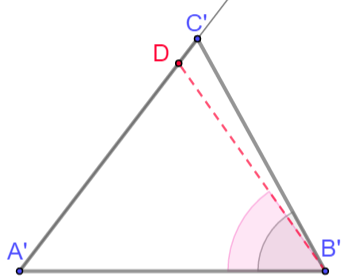
\includegraphics[width=0.35\textwidth]{三角形3.png}
\end{wrapfigure}

注意全等公理包含两种情况。$\angle BAC = \angle B'A'C'$的情况下,两个三角形内角大小一样,
$\angle CBA = \angle C'B'A'$,$\angle ACB = \angle A'C'B'$;另一种情况下,内角的大小总相反,
$\angle CBA = \angle A'B'C'$,$\angle ACB = \angle B'C'A'$。
我们把前者称为\textbf{同角全等},后者称为\textbf{反角全等},分别记为$\simeq$和$\backsimeq$。
如果不强调同角还是反角,可以用$\cong$表示全等。

判定两个三角形全等,还有别的方法。从全等公理还可以得到:
\begin{tm}\label{tm:3-0-0}
    考虑$\triangle ABC$和$\triangle A'B'C'$。如果$|AB| = |A'B'|$,并且$\angle BAC = \angle B'A'C'$、
    $\angle CBA = \angle C'B'A'$成立或$\angle BAC = \angle C'A'B'$、$\angle CBA = \angle A'B'C'$成立,
    那么$\triangle ABC$和$\triangle A'B'C'$全等。    
\end{tm}
\begin{proof2}
    根据等长公理,射线$A'C'$上有一点$D$使得$|A'D| = |AC|$。$\angle BAC = \angle B'A'C'$时,
    根据三角形全等公理,
    $\triangle ABC \simeq \triangle A'B'D$。于是$\angle CBA = \angle DB'A'$。
    而根据条件,$\angle CBA = \angle C'B'A'$,于是射线$B'D$和$B'C'$重合,$D$就是直线
    $B'C'$和$A'C'$的交点。也就是说,点$D$就是点$C'$。因此,
    $\triangle ABC \simeq \triangle A'B'C'$。\\
    $\angle BAC = \angle C'A'B'$时,$\triangle ABC \backsimeq \triangle A'B'D$。
    于是$\angle CBA = \angle A'B'D$,而$\angle CBA = \angle A'B'C'$,从而同样有射线$B'D$和$B'C'$重合,
    因此$\triangle ABC \backsimeq \triangle A'B'C'$。
\end{proof2}
这个定理和全等公理很像。全等公理要求两边和夹角相等,这个定理要求两角和角的公共边相等。
我们把前者简称为“边角边”,后者简称为“角边角”。“角边角”也包含同角和反角两种情况。

\begin{tm}{\textbf{等边对等角}}\label{tm:3-0-1}
    如果三角形的两条边等长(称为\textbf{等腰三角形}),那么它们的对角相等。
\end{tm}
\begin{proof2}
    设有三角形$ABC$,$|AB|=|AC|$。考虑三角形$ACB$,由于$|AB|=|AC|$,$|AC|=|AB|$,$\angle BAC = \angle BAC$,
    根据三角形全等公理,$\triangle ABC \backsimeq \triangle ACB$。于是$\angle ABC = \angle BCA$。
\end{proof2}

等腰三角形可以帮助我们理解等距点的性质。给定两点$A,B$,考虑到两点距离相等的点的集合$\mathfrak{M}$。
首先,线段$AB$的中点$M$属于$\mathfrak{M}$。其次,如果某点$P$属于$\mathfrak{M}$,考虑三角形$ABP$,
它是等腰三角形:$|AP|=|PB|$。因此,根据定理\ref{tm:3-0-1},$\angle PAB = \angle ABP$。

考虑$\triangle MAP$和$\triangle MBP$。$|MA| = |MB|$,$|BP| = |AP|$,$\angle MAP = \angle PBM$,
所以,根据“边角边”,$\triangle MAP \backsimeq \triangle MBP$。于是,$\angle MPA = \angle MPB$。
这说明$\angle MPA$和$\angle MPB$都是直角,直线$MP$垂直于直线$AB$。

反之,如果点$P$使得直线$MP$垂直于直线$AB$,考虑$\triangle MAP$和$\triangle MBP$。
$|MA| = |MB|$,$|MP| = |MP|$,$|\angle AMP| = 90^\circ = |\angle BMP|$。所以,根据“边角边”,
$\triangle MAP \backsimeq \triangle MBP$。于是$|AP| = |BP|$,即$P\in\mathfrak{M}$。

总结下来,就是:
\begin{tm}{\textbf{垂直平分线定理}}\label{tm:3-0-2}
    到两点$A,B$距离相等的点的集合,是过线段$AB$中点且与它垂直的直线,称为两点的\textbf{垂直平分线}或\textbf{中垂线}。
\end{tm}

垂直平分线可以帮我们把一个角平分成两半。给定一个角,可以在它始边上和终边上各找一点$A,B$,使得角的顶点$O$到
这两点距离相等。于是$\triangle AOB$是等腰三角形。考虑线段$AB$的中点$M$,前面我们已经证明了:
$\triangle MAO \backsimeq \triangle MBO$。所以,$\angle AOM = -\angle BOM$。这说明$\angle AOB = 2\angle AOM$。
我们说点$M$或射线$OM$\textbf{平分}$\angle AOB$。$OM$称为$\angle AOB$的\textbf{角平分线},它把$\angle AOB$平分成两半。


\begin{wrapfigure}{r}{0.33\textwidth} %this figure will be at the right
    \vspace{-15pt}
    \centering
    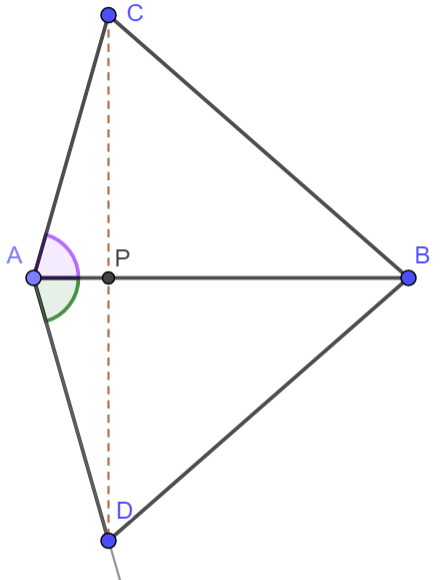
\includegraphics[width=0.33\textwidth]{三角形4.png}
\end{wrapfigure}

利用垂直平分线的性质,还可以证明另一种判定三角形全等的方法:
\begin{tm}\label{tm:3-0-4}
    如果$\triangle ABC$和$\triangle A'B'C'$满足$|AB| = |A'B'|$,$|AC| = |A'C'|$,$|BC| = |B'C'|$,
    那么$\triangle ABC$和$\triangle A'B'C'$全等。
\end{tm}
\begin{proof2}
    作射线$AD$使得$|\angle DAB| = |\angle C'A'B'|$并且与$\angle BAC$异号,并使$|AD| = |A'D'|$。
    这样得到的点$D$和$C$分处直线$AB$两侧。
    由于$|AB| = |A'B'|$,根据“边角边”,$\triangle ABD \cong \triangle A'B'C'$。\\
    考察$\triangle ABC$和$\triangle ABD$。$|AC| = |A'C'| = |AD|$,所以$A$在线段$CD$的垂直平分线上。\\
    作辅助线$CD$,交直线$AB$于点$P$。$\triangle APC \backsimeq \triangle APD$。于是$\angle PAC = -\angle PAD$,从而
    $\angle BAC = -\angle BAD$。
    因此,根据“边角边”,$\triangle ABC \cong \triangle ABD \cong \triangle A'B'C'$。
\end{proof2}

这个定理告诉我们,三边都对应相等的两个三角形是全等三角形。我们把这个结论简称为“边边边”。
由于条件中没有角的情况,我们无法确定是同角全等还是反角全等。

综上,我们有三个判定三角形全等的方法:“边角边”、“角边角”和“边边边”。

\begin{wrapfigure}[4]{r}{0.6\textwidth} %this figure will be at the right
    \vspace{-15pt}
    \centering
    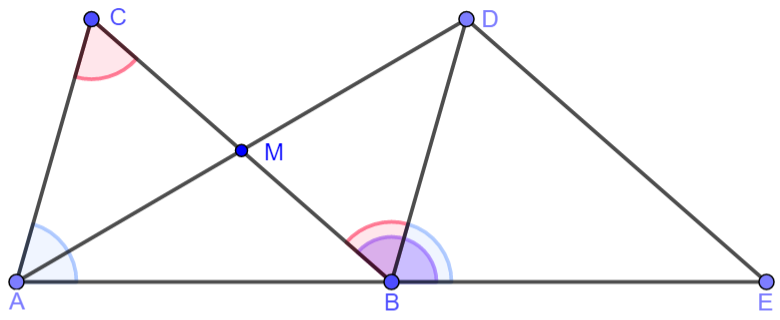
\includegraphics[width=0.6\textwidth]{三角形5.png}
\end{wrapfigure}

三角形全等可以用来证明三角形的基本性质。

\begin{tm}\label{tm:3-0-5}
    三角形的外角是另外两个内角的和。
\end{tm}

\begin{proof2}
    如右图,我们想证明$\angle CBA$的外角等于$\angle BAC + \angle ACB$。\\
    在射线$AB$上找一点$E$,使得$|AB| = |BE|$。作线段$BC$的中点$M$,在射线$AM$上找一点$D$,
    使得$|AM| = |MD|$。
    我们接下来会证明$\angle EBD = \angle BAC$以及$\angle DBC = \angle ACB$。
    这样的话,就得到
    $$\angle BAC + \angle ACB = \angle EBD + \angle DBC = \angle EBC,$$
    而$\angle EBC$就是$\angle CBA$的外角。\\
    我们首先证明$\triangle MCA \cong \triangle MBD$。\\
    $M$是线段$BC$的中点,因此,$|MC| = |MB|$。$\angle CMA$和$\angle BMD$是对顶角,所以相等。
    再加上$|AM| = |MD|$,根据“边角边”,$\triangle MCA \cong \triangle MBD$。
    因此,$\angle DBC = \angle ACB$,且$|BD| = |AC|$。\\
    接下来,我们证明$\triangle ABC \cong \triangle BED$。\\
    从$A$出发的两条射线$AE$和$AD$上分别有点$B,E$和$M,D$,且
    $$ \frac{|AB|}{|AE|} = \frac{|AM|}{|AD|} = \frac12,$$
    因此,根据放缩公理,
    $$ \frac{|BM|}{|DE|} = \frac12.$$
    也就是说,$|DE| = 2|BM| = |BC|$。而我们已知$|BE| = |AB|$,$|BD| = |AC|$。
    所以,根据“边边边”,$\triangle ABC \cong \triangle BED$。于是,$\angle EBD = \angle BAC$。
\end{proof2}
从这个定理,我们可以推出:三角形三个内角之和等于平角。这个结论,我们已经有直观感受。现在,我们从公理出发,
严格证明了这个结论。

\section{垂直和垂线}

\begin{wrapfigure}[5]{r}{0.3\textwidth} %this figure will be at the right
    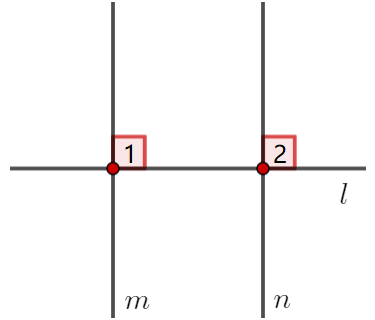
\includegraphics[width=0.3\textwidth]{三角形6.png}
\end{wrapfigure}
垂直平分线定理告诉我们,到两点距离相等的点构成一条直线,它和两点所在的直线垂直。通过垂直平分线定理,
我们可以了解更多与垂直有关的性质。

\begin{tm}{\textbf{垂直定理}}\label{tm:3-1-0}
    垂直于同一直线的两条直线平\\
    行或重合。
\end{tm}
\begin{proof2}
    设直线$m,n$都垂直于直线$l$。\\
    如果$m,n$分别与$l$相交于不同的两点,如右图,$\angle 1$和$\angle 2$都是直角,
    而且是同位角。于是根据同位角的性质,$m \parallel n$。\\
    如果$m,n$与$l$相交于同一点$O$,以$l$在$O$任一侧的射线为始边,以$m$在$O$的任一侧为终边,形成的角是直角;
    同样,以$n$在$O$的任一侧为终边,形成的也是直角。因此它们的终边重合。也就是说,直线$m,n$重合。
\end{proof2}
类似的结论还有:
\begin{itemize}
    \item 如果直线$m \parallel n$,$n \perp l$,那么$m \perp l$。
    \item 如果直线$m \perp n$,$n \parallel l$,那么$m \perp l$。
    \item 如果直线$m \parallel n$,直线$l_1 \perp m$,$l_2 \perp n$,那么$l_1$与$l_2$平行或重合。
\end{itemize}
\begin{tm}{\textbf{垂线定理}}\label{tm:3-1-1}
    过一点有唯一的直线与给定直线垂直,称为点到给定直线的\textbf{垂线}。
\end{tm}
\begin{proof2}
    设有直线$l$和点$P$,我们要找一条直线$m$,使得$P$在$m$上,且$m\perp l$,并且要证明这样的直线只有一条。\\
    首先找到这样的直线$m$。过$l$上两点,可以作垂直平分线$p$,按定义$p \perp l$。\\
    如果$P$在$p$上,那么$m=p$。如果$P$不在$p$上,那么过$P$有唯一直线$m$与$p$平行。于是$m\perp l$。\\
    再证明这样的直线是唯一的。设$m$和$l$相交于点$H$,在$l$上找另一点$A$,作$AH$的垂直平分线$n$。$n\perp l$,而且$H$不在$n$上,
    所以$n \parallel m$,且$P$不在$n$上。如果过$P$的直线垂直于$l$,那么它平行于$n$,根据平行公理,这样的直线是唯一的。
\end{proof2}
我们把垂线$m$与直线$l$的交点$H$称为$P$或$m$到$l$的\textbf{垂足}。

\begin{tm}{\textbf{角平分线定理}}\label{tm:3-1-20}
    作$\angle AOB$的角平分线上任一点$P$到角的始边和终边的垂线,垂足分别为$A$和$B$,则$|PA| = |PB|$
\end{tm}
\begin{proof2}
    $\triangle APO$和$\triangle BPO$都是直角三角形。$\angle PAO$和$\angle PBO$都是直角。
    而$OP$平分$\angle AOB$,所以$\angle AOP = \angle POB$。因此第三个角也相等:$\angle APO = \angle OPB$。
    两个三角形有共同的边$|PO| = |PO|$,根据“角边角”,$\triangle APO \backsimeq \triangle BPO$。
    于是$|PA| = |PB|$。
\end{proof2}
这个定理可以简单说成:角平分线上的点到两边距离相等。角平分线定理的证明中$\triangle APO \backsimeq \triangle BPO$,
所以还可以得出$|AO| = |BO|$。

\begin{xt}
    证明垂直定理的推论:\\
    \indent 1. 如果直线$m \parallel n$,$n \perp l$,那么$m \perp l$。\\
    \indent 2. 如果直线$m \perp n$,$n \parallel l$,那么$m \perp l$。\\
    \indent 3. 如果直线$m \parallel n$,直线$l_1 \perp m$,$l_2 \perp n$,那么$l_1$与$l_2$平行或重合。\\
    证明角平分线定理的逆定理:\\
    \indent 到角的始边和终边距离相等的点,都在角平分线上。
\end{xt}

\chapter{特殊三角形}
我们之前定义了等腰三角形。等腰三角形和等距点有密切关系,是我们理解三角形性质的有力工具。
接下来,我们会继续了解等腰三角形的性质,并且了解另外几种特殊的三角形。

\section{等腰三角形}
等腰三角形是有两边相等的三角形。定理\ref{tm:3-0-1}告诉我们,两边相等,对应的角也相等。
我们把相等的两边称为\textbf{腰},把第三边称为\textbf{底}或\textbf{底边},把腰的对角称为\textbf{底角},
把底边的对角称为\textbf{顶角}。

给定等腰三角形$ABC$,其中$\angle A$为顶角。$\angle A$的平分线与底边的交点称为\textbf{中足}。
记中足为$M$,由于$\angle MAB = \angle CAM$,
$\angle CBA = \angle ABC$,所以$\angle AMB = \angle CMA$。
这说明$\angle AMB = \angle CMA = 90^\circ$。可以推出$\triangle AMC \backsimeq \triangle AMB$。
也就是说,$AM$是$BC$的垂直平分线。因此,$M$是线段$BC$的中点。

\begin{tm}{\textbf{等角对等边}}\label{tm:4-0-0}
    如果三角形有两内角相等,那么它们对边也相等。
\end{tm}
\begin{proof2}
    设$\triangle ABC$中$\angle CBA$和$\angle ACB$相等。考虑$\triangle ACB$。
    $\angle CBA = \angle ACB$,$\angle ACB = \angle CBA$,$|BC| = |CB|$,所以根据“角边角”,
    $\triangle ABC \backsimeq \triangle ACB$,因此$|AB| = |AC|$。
\end{proof2}

定理\ref{tm:3-0-1}和\ref{tm:3-1-0}称为\textbf{互逆命题}。它们互为对方的\textbf{逆命题}。
逆命题一般针对假言命题。把假言命题中的前件和后件互换,就得到它的逆命题。
比如,“如果点在线段的垂直平分线上,那么它到线段两端距离相等”的逆命题是:
“如果点到线段两端距离相等,那么它在线段的垂直平分线上”。

一个命题是真的,它的逆命题不一定是真的。比如,“如果两个角是对顶角,那么它们相等”是真的;
但它的逆命题:“如果两个角相等,那么它们是对顶角”是假的。
反之,一个命题的逆命题是真的,它自身也不一定是真的。

把命题中的判断换成非判断,得到的命题叫做\textbf{否命题}。比如,假言命题“如果点在线段的垂直平分线上,那么它到线段两端距离相等”
的否命题是“如果点不在线段的垂直平分线上,那么它到线段两端距离不相等”。
简单命题的否命题,真假和原命题恰好相反。对复合判断,否命题的真假和原命题不一定相反。

假言命题的否命题的逆命题,就是先把前件和后件中的判断都改成非判断,再把前件和后件互换。
要注意的是,假言命题的否命题的逆命题,和假言命题的逆命题的否命题是一样的。
因为前后件互换和同时把前后件变成非判断这两个操作互相并不妨碍。这样得到的命题称为原来的假言命题的\textbf{逆否命题}。
比如,“如果点在线段的垂直平分线上,那么它到线段两端距离相等”的逆否命题是
“如果点到线段两端距离不相等,那么它不在线段的垂直平分线上”。

\begin{sk}\label{sk:4-0-0}
    \mbox{}\\
    以下命题对吗?你能否证明?它们的逆命题和逆否命題是什么?\\
    \indent 1. 如果三角形某个顶点和对边中点确定的直线平分顶点所在的内角,那么三角形是等腰三角形。\\
    \indent 2. 如果三角形某个顶点与对边中点确定的直线垂直于对边,那么三角形是等腰三角形。\\
    \indent 3. 如果三角形某内角的平分线过对边的中点,那么三角形是等腰三角形。\\
    \indent 4. 如果三角形某内角的平分线与对边垂直,那么三角形是等腰三角形。\\
    \indent 5. 如果三角形某个顶点到对边的垂线过对边中点,那么三角形是等腰三角形。\\
    \indent 6. 如果三角形某个顶点到对边的垂线平分顶点所在的内角,那么三角形是等腰三角形。\\
    满足什么条件时,两个等腰三角形全等?\\
\end{sk}

我们把三边都相等的三角形称为\textbf{等边三角形},把三个内角都相等的三角形称为\textbf{等角三角形}。
通过定理\ref{tm:3-0-1}和\ref{tm:3-1-0}可以知道,这两种三角形是一种三角形。

等边三角形是特殊的等腰三角形。它的三个内角都是$60^\circ$,三个外角都是$120^\circ$。
它每个内角的平分线都垂直于对边并过对边中点,把自己分成两半。

\begin{xt}\label{xt:4-0-0}
    证明:\\
    \indent 1. 有一个内角是$60^\circ$的等腰三角形是等边三角形。\\
    \indent 2. 等腰三角形三边的垂直平分线交于一点。\\
    \indent 3. 从等腰三角形每个顶点向对边作垂线,三条垂线交于一点。\\
    \indent 4. 连接等腰三角形每个顶点和对边中点作直线,三条线交于一点。\\
    \indent 5. 等腰三角形三个内角的平分线交于一点。
\end{xt}

\section{直角三角形}
三个内角中有一个是直角的三角形称为直角三角形。学习垂直平分线、等腰三角形时,
我们已经见过直角三角形了。现在我们来单独了解它的性质。

直角三角形有一个内角是直角,因此,另外两个角之和也等于直角。
直角的对边叫做\textbf{斜边}或\textbf{弦},直角的邻边叫做\textbf{直角边}。

\begin{tm}\label{tm:4-1-0}
    直角三角形斜边长度是直角顶点到斜边中点距离的两倍。
\end{tm}
\begin{proof2}
    设直角三角形$AOB$中$\angle O$是直角。记斜边$AB$中点为$M$,直角边$OA$中点为$N$。
    连接$OM$、$MN$。射线$AB$、$AO$上有:
    $$ \frac{|AN|}{|AO|} = \frac{|AM|}{|AB|} = \frac12.$$
    根据放缩公理,$MN \parallel OB$。因此$MN \perp OA$。这说明$MN$是线段$OA$的垂直平分线。
    因此$|OM| = |AM|$,$|AB| = 2|AM| = 2|OM|$。
\end{proof2}
可以观察到,斜边中点和直角顶点的连线(称为斜边上的中线)是两条直角边的垂直平分线的交点。
$\triangle MOB$、$\triangle MOA$都是等腰三角形。

两个直角三角形全等的判定条件,比一般的三角形要简单。毕竟,我们已经知道它们某个角相等了。

\begin{tm}\label{tm:4-1-1}
    两个直角三角形斜边等长,且有一条直角边等长,那么它们是全等三角形。
\end{tm}
\begin{proof2}
    设直角$\triangle ABC$和$\triangle A'B'C'$满足:斜边$|BC| = |B'C'|$,直角边$|AC| = |A'C'|$。
    延长线段$BA$,在直线$BA$上找一点$D$使得$|AD| = |A'B'|$,并且$B,D$处于$A$的两侧。
    $\angle DAC$是直角$\angle CAB$的补角,因此也是直角。根据“边角边”,
    $\triangle DAC \cong \triangle B'A'C'$。于是,$|DC| = |B'C'| = |BC|$。这说明点$C$在线段$BD$的垂直平分线上。
    而$CA \perp BD$,所以$AC$就是线段$BD$的垂直平分线。这说明$A$是$BD$的中点。$|AB| = |AD|$。
    因此根据“边角边”,$\triangle ABC \cong \triangle ADC \cong \triangle A'B'C'.$
\end{proof2}

如果一个三角形既是等腰三角形,又是直角三角形,就称它是\textbf{等腰直角三角形}。
等腰直角三角形的腰只能是直角边,也就是说,顶角是直角。两个底角之和是直角,所以底角是$45$度角。
换句话说,所有等腰直角三角形长得都一样。

\begin{sk}\label{sk:4-1-0}
    \mbox{}\\
    以下命题对吗?你能否证明?\\
    \indent 1. 两个直角三角形有一个锐角相等,该角的对边等长,那么这两个三角形全等。\\
    \indent 2. 两个直角三角形有一个锐角相等,且斜边等长,那么这两个三角形全等。\\
    \indent 3. 两个直角三角形有一个锐角相等,且该角的直角边等长,那么这两个三角形全等。\\
    \indent 4. 两个直角三角形的两个直角边分别等长,那么这两个三角形全等。\\
    \vspace{2pt}\\
    设$\triangle ABC$是直角三角形,$\angle BAC$是直角。过$A$作关于$BC$的垂线,垂足为$H$,思考以下问题:\\
    \indent 1. $\triangle AHB$、$\triangle AHC$、$\triangle ABC$之间有什么关系?\\
    \indent 2. 能否用$AB, BC, CA$表达线段$BH$和$CH$的长度?\\
    \indent 3. 能不能用一个简单的等式表示$AB, BC, CA$长度之间的关系?
\end{sk}


\chapter{整数的性质}

\section{整除和同余}
如果整数$m$能写成整数$n$和整数$q$的乘积,就说$n$整除$m$,$m$是$n$的倍数,$n$是$m$的因数。
一般的情况下,总有自然数$r < n$和整数$q$,使得:
$$ m = nq + r.$$
这就是整数的带余除法。我们说$r$是$m$除以$n$得到的余数,$m$和$r$模$n$同余,记作:
$$ m \equiv r \mod n.$$

一般来说,两个整数$a$和$b$相差$n$的倍数,就说它们模$n$同余。比如$4$和$9$模$5$同余。
给定整数$n$,任何两个整数要么模$n$同余,要么模$n$不同余,而且:
\begin{enumerate}
    \item $\forall a \in \mathbb{Z}, \quad a \equiv a \mod n.$
    \item $a \equiv b \mod n$,当且仅当$b \equiv a \mod n.$
    \item 如果$a \equiv b \mod n$且$b \equiv c \mod n$,那么$a \equiv c \mod n.$
\end{enumerate}
所有模$n$同余的整数的集合称为模$n$的\textbf{同余类}。比如,所有除以$5$余$1$的整数的集合就是一个模$5$的同余类。
同样地,除以$5$余$0$、$2$、$3$、$4$的整数的集合各是模$5$的同余类。模$5$的同余类一共有$5$个。一般来说,
模$n$的同余类有$n$个,分别是除以$n$余$0,1,\cdots,n-1$的整数的集合。为了方便,我们把这些同余类记作:
$$ \overline{0}, \overline{1}, \cdots , \overline{n-1}.$$

\section{辗转相除法}
因数只有自己和$1$的正整数叫做\textbf{素数},除了$1$和自己还有别的因数的正整数叫做\textbf{合数}。我们约定$1$既不是素数也不是
合数。

举例来说,$2$、$3$、$5$、$7$是素数,而$4$、$6$、$8$是合数。偶素数只有一个:$2$,其余素数都是奇数。

如果整数$p$既是整数$n$的因数,又是整数$m$的因数,那么就说$p$是$n$和$m$的\textbf{公因数}。同理,
如果整数$p$既是整数$n$的倍数,又是整数$m$的倍数,那么就说$p$是$n$和$m$的\textbf{公倍数}。
显然,对任何两个整数$n,m$来说,$1$总是它们的公因数,$nm$总是它们的公倍数。我们更关心$n,m$的公因数中最大的数,
和公倍数中最小的数。它们分别叫做整数$n,m$的最大公因数和最小公倍数。

如果两个数的最大公因数是$1$,就说它们\textbf{互素}。

如何求整数$n,m$的最大公因数?不妨设$n\leqslant m$(否则把它俩换个顺序)。如果$m$是$n$的倍数,那么$n$就是它们的最大公因数。
如果$m$不是$n$的倍数,那么我们考虑$m$除以$n$得到的余数$r$。设$m = nq + r$。设$d$是$n,m$的公因数,
那么有整数$a,b$使得$m = ad$,$n = bd$。于是
$$ d(a - nb) = r.$$
这说明$d$也是$r$的因数。反过来,如果$d$是$n$和$r$的公因数,整数$b, c$使得$n = bd$,$r = cd$,那么$m = (nb + c)d$,
于是$d$也是$m$的因数。
这说明$n,m$的最大公因数就是$r,n$的最大公因数。

这样,我们可以把求整数$n,m$最大公因数的目标改为求$r,n$的最大公因数。根据余数的定义,$r < n$。
所以,经过这样一步转化,我们要处理的数更小了,目标却没有变。

这样一步步下来,每一步之后,两个数里较大的数比前一步至少减少了$1$。所以,要么在某一步时我们发现一个数是另一个的倍数,
这样就求出了最大公因数;要么经过至多$m-1$步后,两个数最终都小于$2$,因此一个是$0$,一个是$1$。这时最大公因数就是$1$。

这个求最大公因数的方法,称为\textbf{辗转相除法}。给定整数$n\leqslant m$,
\begin{enumerate}
    \item $m$对$n$做带余除法:$m = q n + r$。
    \item 如果$r = 0$,那么最大公因数就是$n$。
    \item 如果$r > 0$,那么对$r$和$n$重复步骤$1$。
\end{enumerate}

\begin{xt}\label{xt:5-2-0}
    辗转相除法中,\\
    \indent 1. 为什么$n,m$的最大公因数就是$n,r$的最大公因数?\\
    \indent 2. 为什么每步之后,两个数里较大的数比前一步时至少减少了$1$?\\
    算一算:\\
    \indent 1. 用辗转相除法求$376$和$488$的最大公因数。\\
    \indent 2. 用辗转相除法求$144$和$209$的最大公因数。
\end{xt}

\section{更相分益法}
使用辗转相除法求$42$和$60$的最大公因数:
\begin{enumerate}
    \item $60 = 1 \times 42 + 18$,转为求$18$和$42$的最大公因数。
    \item $42 = 2 \times 18 + 6$,转为求$6$和$18$的最大公因数。
    \item $18 = 3 \times 6$,所以最大公因数是$6$。
\end{enumerate}
把这个过程反过来,我们得到:
\begin{align}
    6 &= 42 - 2 \times 18 \notag \\
    &= 42 - 2 \times (60 - 1 \times 42) \notag \\
    &= (1 + 2\times 1) \times 42 + (-2) \times 60 \notag 
\end{align}
我们把$42$和$60$的最大公因数$6$用$42$和$60$的倍数表示了出来。一般来说,我们也可以这么做。
\begin{tm}{\textbf{倍和析因定理}}\label{tm:5-2-0}
    可以用两个整数$n,m$的倍数之和表示它们的最大公因数。
\end{tm}
\begin{proof2}
    先用辗转相除法,$k$步求出整数$n,m$的最大公因数$d$。设每步处理的两个数分别是$n_1=n,n_0=m$、$n_2, n_1$、$n_3, n_2$,直到$n_k, n_{k-1}$。
    于是$d = n_k$。\\
    辗转相除法最后一步可以改写为$n_{k-1} = sd $。倒数第二步可以写成$n_{k-2} = q_{k-1}n_{k-1} + d$,
    因此$d = n_{k-2} -q_{k-1}n_{k-1}$。也就是说,$d$可以表示为$n_{k-2}$和$n_{k-1}$的倍数的和,。\\
    再往前一步,有$n_{k-3} = q_{k-2}n_{k-2} + n_{k-1}$。
    于是$n_{k-1} = n_{k-3} - q_{k-2}n_{k-2}$可以表示为$n_{k-3}$和$n_{k-2}$倍数的和,
    因而可以把$d$写成:
    $$d = n_{k-2} - q_{k-1}n_{k-1} = n_{k-2} - q_k(n_{k-3} - q_{k-2}n_{k-2}).$$
    $d$可以表示为$n_{k-3}$和$n_{k-2}$倍数的和。\\
    如此进行下去,$k$次后,就能把$d$表示成$n_1,n_0$(也就是$n,m$)倍数的和。
\end{proof2}
这个方法叫做\textbf{更相分益法}。简单来说,就是把辗转相除法倒过来。

如果$n,m$互素,倍和析因定理告诉我们,可以找到它们的倍数,相加为$1$。

\begin{xt}\label{xt:5-2-1}
    算一算:\\
    \indent 1. 用更相分益法把$376$和$488$的最大公因数表示成它们倍数的和。\\
    \indent 2. 用更相分益法把$144$和$209$的最大公因数表示成它们倍数的和。
\end{xt}

\end{document}